%\documentclass[mathserif,xcolor=dvipsnames]{beamer}
\documentclass[xcolor=dvipsnames]{beamer}

%\usefonttheme{serif}
%\setbeamerfont{structure}{family=\sffamily,shape=\upshape} 

\usefonttheme{professionalfonts}

\usepackage{math}
\usepackage{util}
\usepackage{ufont}

\usetheme{Madrid}
%\usecolortheme[named=RawSienna]{structure} 
\usecolortheme[named=MidnightBlue]{structure} 
\useoutertheme{umbcfootline} 
%\usetheme[height=7mm]{Rochester} 
\setbeamertemplate{items}[ball] 
\setbeamertemplate{blocks}[rounded][shadow=true] 
\setbeamertemplate{navigation symbols}{} 

\newcommand*{\as}{A}
\newcommand*{\ms}{\mathcal M}


%\title[The Geometry of DBNs]{The (Real) Geometry of \\the Restricted Boltzmann Machine}
\title[Symmetric Binary Models]{Algebraic Statistics and Symmetric Binary Models}
\author{Aaron Pribadi}
\institute[HMC]{Harvey Mudd College \\ PCUMC}
\date{March 10, 2012}

\begin{document}

\begin{frame}[plain]
    \maketitle
\end{frame}


\begin{frame}{Binary Data}

    \begin{columns}

    \begin{column}{0.5\textwidth}
        The votes of 376 members of the U.S. House of Representatives on
        four selected bills.  
        
        \lspace
        Data are from the UCI Machine Learning Repository.
    \end{column}

    \begin{column}{0.5\textwidth}
    \begin{center}
    \begin{tabular}{c c}
        Voting Record & Counts \\
        \hline
        \only<1>{NNNN}\only<2>{0000} & 6 \\
        \only<1>{NNNY}\only<2>{0001} & 54 \\
        \only<1>{NNYN}\only<2>{0010} & 38 \\
        \only<1>{NNYY}\only<2>{0011} & 8 \\
        \only<1>{NYNN}\only<2>{0100} & 5 \\
        $\vdots$ & $\vdots$ \\
        \only<1>{YYYY}\only<2>{1111} & 5 
        \\
        \\
        & 376 Total
    \end{tabular}
    \end{center}
    \end{column}

    \end{columns}

        
    \lspace
    {\footnotesize
    \texttt{http://archive.ics.uci.edu/ml/datasets/Congressional+Voting+Records}
    }

\end{frame}

\begin{frame}{Binary Data}
    Assumption: The data points are i.i.d. random variables.
    \[
        X_1, X_2, \ldots, X_{376}
        \qquad
        \text{with $X_i$ taking values in $\{0, 1\}^4$}
    \]

    \lspace
    Big question: What is the underlying probability distribution of $X_i$?
\end{frame}

\begin{frame}{Statistical Models, Geometrically}
    There are $\vdel[\big]{\{0, 1\}^4} = 2^4 = 16$ states: \quad $s_k = 0000, 0001,
    0010, \ldots$
    \[
        p_k = P[X = s_k]
        \qquad
        \text{where $\sum_{k=1}^{16} p_k = 1$ and $p_k \ge 0$}
    \]
\end{frame}
\begin{frame}{Statistical Models, Geometrically}
    \lspace
    \lspace
    The $(N-1)$-dimensional \textbf{probability simplex} is the space
    \[
        \Delta_{N-1} = \cdel*{ (p_1, \ldots, p_N) \:: \sum_k p_k= 1, p_k \ge 0 }
        \subset \R^N
    \]
    \nlspace
    \begin{figure}\centering
        \includegraphics[width=0.2\textwidth]{2-simplex.pdf} 
        \caption{The 2-simplex}
    \end{figure}
\end{frame}

\begin{frame}{Statistical Models, Geometrically}
    A \textbf{statistical model} is a subset $\ms \subset \Delta$ of the
    simplex.

    \lspace
    We only care about \emph{some} of the probability distributions.

    \pause
    \lspace
    \begin{example}
        The binomial distribution is a model with the following parametrization.
        \begin{align*}
            [0, 1] &\to \ms \\
            \lambda &\mapsto (p_0, \ldots, p_n)
            \qquad
            \text{with}
            \qquad
            p_k = \binom n k \lambda^k (1 - \lambda)^{n-k}
        \end{align*}
    \end{example}
\end{frame}

\begin{frame}{Log-Linear Models}
    \textbf{log-linear model}: The log of the model is in a linear space $V$.
    \[
        \ms_V = \cdel[\big]{ p \in \Delta_{N-1}
        \::\: \log p  = (\log p_1, \ldots, \log p_N) \in V}
    \]

    \lspace
    \lspace
    {\footnotesize
    (Note: $p_k > 0$, and $V$ must intersect the positive quadrant.)
    }
\end{frame}

\begin{frame}{Log-Linear Models}
    \lspace
    One way to specify a log-linear model is with a matrix $\as \in \Z^{d
    \times N}$.
    \[
        \ms_\as = \cdel[\big]{ p \in \Delta_{N-1}
        \:: \log p  \in \mathrm{rowspace}(\as)}
    \]

    \pause
    \begin{example}
    \[
        \as = \kbordermatrix{
            & 00 & 01 & 10 & 11 \\
            &  1 & 1  & 0  & 0 \\
            &  0 & 0  & 1  & 1 \\
            &  1 & 0  & 1  & 0 \\
            &  0 & 1  & 0  & 1
        }
        \qquad
        \text{\footnotesize Not full rank.}
    \]
    \end{example}

    {\footnotesize
        (Note: Non-negative entries, columns sum to same value.)
    }
\end{frame}

\begin{frame}{Log-Linear Models}
    Lots of familiar examples.
    \begin{example}[Independence Model]
    \[
        \as = \kbordermatrix{
            & 00 & 01 & 10 & 11 \\
            &  1 & 1  & 0  & 0 \\
            &  0 & 0  & 1  & 1 \\
            &  1 & 0  & 1  & 0 \\
            &  0 & 1  & 0  & 1
        }
        \qquad
        \ms_\as = \cdel[\big]{ p \in \Delta_{N-1}
        \:: \log p  \in \mathrm{rowspace}(\as)}
    \]
    A distribution is in $\ms_\as$ if its first and second bits are independent.
    \end{example}
\end{frame}

\begin{frame}{Log-Linear Models}
    \begin{example}[Markov Random Fields]
    `Undirected graphical models'
    \begin{figure}\centering
        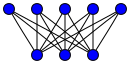
\includegraphics[width=0.4\textwidth]{bipartite.pdf} 
        \caption{Independence graph of the Restricted Boltzmann
        Machine.}
    \end{figure}
    \end{example}
\end{frame}

\begin{frame}{Selecting a Model}
    How good is a model?

    \lspace
    The \textbf{maximum likelihood estimate} $\hat p \in \ms$
    maximizes the log-likelihood
    \[
        l(p) = \log \pdel*{\prod_{i=1}^m P[X_i = x_i]}.
    \]
    `Want to make the data more likely.'
\end{frame}

\begin{frame}{Polynomials!}
    Parametric map $\phi_A: \R_{>0}^d \to \ms_A$
    \[
        \phi_\as(\theta) = 
        \pdel*{
            \theta_1^{a_{11}} \cdots
            \theta_d^{a_{d1}}
            ,\;\ldots\;,
            \theta_1^{a_{1N}} \cdots
            \theta_d^{a_{dN}}
        }
    \]

    \lspace 
    Now for a tiny bit of algebraic geometry \ldots

    \lspace
    \lspace
    {\footnotesize
        (Note: Must normalize the map.)
    }
\end{frame}

\begin{frame}{Affine Varieties}
    An \textbf{affine algebraic set} is the zero-set
    \[
        V(f_1, \ldots, f_m) = 
        \cdel[\big]{
        x \in \mathbb K^n \::
        f_i(x) = 0 \qquad
        \text{for all $i$}
        }
    \]
    of some polynomials $f_i \in \mathbb K[x_1, \ldots, x_n]$.

    \lspace
    \lspace
    The \textbf{vanishing ideal} of a set $V \subset \mathbb K^n$ has
    the polynomials
    \[
        I(V) = \cdel[\big]{f \in \mathbb K[x_1, \ldots, x_n] \::
        f(x) = 0 \qquad
        \text{for all $x \in V$}}.
    \]
\end{frame}

\begin{frame}{Toric Ideal}
    The vanishing ideal of a log-linear model has a nice generating set.
    \[
        I_\as = I(\ms_\as) = \adel[\big]{
            p^u - p^v \::
            \text{$u, v \in \mathbb N^d$ and $\as u = \as v$}
        }
    \]

    \lspace
    \lspace
    \lspace
    {\footnotesize
        (Note: You often work with the Zariski closure, which is a toric
        variety.)
    }
\end{frame}

\begin{frame}{Computing Maximum Likelihood}
    \begin{theorem}[Birch's Theorem]
        The maximum likelihood estimate for a log-linear model $\ms_\as$ with
        data $X_1, \ldots, X_m$ summarized as a count $u \in \mathbb{N}^N$ is
        the unique solution non-negative solution to the equations
        \[
            \as (mp) = \as u
            \qquad\text{and}\qquad
            p \in V(I_\as)
        \]
    \end{theorem}

    \lspace
    \lspace
    {\footnotesize
        (Note: $u$ must be strictly positive.)
    }
\end{frame}

\begin{frame}{Another Way to Select a Model}
    Does the data look `typical' for the model?

    \lspace

    \begin{theorem}[Sufficient Statistic]
        Conditioned on a sufficient statistic $\as u$, the distribution of
        counts does not depend on the parameter.
        \[
            P[U = u \mid \as U = \as u, p \in \ms_\as]
            =
            P[U = u \mid \as U = \as u]
        \]
    \end{theorem}

    There exists an algorithm (Metropolis-Hastings) to sample from $U$ using
    the conditional distribution $P[U = u \mid AU = Au]$.

    \lspace
    You need a \textbf{Markov basis} for $A$.
\end{frame}

\begin{frame}{Monte Carlo Markov Chain}
    \begin{theorem}[Fundamental Theorem of Markov Bases]
        A set of moves $\{b_1, \ldots, b_k\}$ with $b_i \in \Z^N$ is a Markov basis
        if and only if the corresponding set of binomials $\{p^{b_i^+} -
        p^{b_i^-}\}$ generates the ideal $I_A$.
    \end{theorem}
\end{frame}

\begin{frame}{Symmetric Models}
    What kind of models should we consider?

    \lspace
    Random variable $X$ with values in $\{0, 1\}^n = \{0\cdots00, 0\cdots01,
    \ldots, 1\cdots11\}$.

    \lspace
    Two natural symmetry requirements:
    \begin{itemize}
    \item The model is invariant under permuting the bits.
    \item The model is invariant under flipping any bit.
    \end{itemize}
\end{frame}

\begin{frame}{Symmetric Models}
    These operations generate the \textbf{hyperoctahedral group} $S_2 \wr S_n$.

    \lspace
    You can think of it as permuting the vertices of a hypercube.
    \begin{figure}[h]
        \centering
        % http://code.google.com/p/graph-theory-algorithms-book/
        % GPL Documentation Licence

        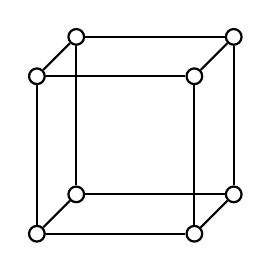
\begin{tikzpicture}
        [nodedecorate/.style={shape=circle,inner sep=2pt,draw,thick},%
          linedecorate/.style={-,thick}]
        %% nodes or vertices
        \foreach \nodename/\x/\y in {1/0/0, 2/2/0, 3/2/2, 4/0/2, 5/0.5/0.5,
          6/2.5/0.5, 7/2.5/2.5, 8/0.5/2.5}
        {
          \node (\nodename) at (\x,\y) [nodedecorate] {};
        }
        %% edges or lines
        \path
        \foreach \startnode/\endnode in {1/2, 2/3, 3/4, 4/1, 5/6, 6/7, 7/8,
          8/5, 1/5, 2/6, 3/7, 4/8}
        {
          (\startnode) edge[linedecorate] node {} (\endnode)
        };
        \end{tikzpicture}

        \caption{The $3$-hypercube graph}
        \label{fig:hypercube}
    \end{figure}
\end{frame}

\begin{frame}{Symmetric Models}
    Remember what a log-linear model look like: 
    \[\ms_V = \cdel[\big]{ p \in \Delta_{N-1} \:: \log
    p  \in V}\]

    \lspace
    The space $V \subset \R^N$ must be invariant under the action of $S_2 \wr
    S_n$.
\end{frame}

\begin{frame}{Symmetric Models}
    From representation theory, we know that $V$ must decompose into irreducible
    invariant subspaces
    \[
        V = V_1 \oplus \cdots \oplus V_k.
    \]
\end{frame}

\begin{frame}{Symmetric Models}
    The group $S_2 \wr S_n$ is nice; its permutation representation breaks up into
    the eigenspaces of the adjacency matrix of the hypercube graph.
    \[
        \kbordermatrix{
            & 00 & 01 & 10 & 11 \\
        00  &  0 & 1  & 1  & 0 \\
        01  &  1 & 0  & 0  & 1 \\
        10  &  1 & 0  & 0  & 1 \\
        11  &  0 & 1  & 1  & 0
        }
    \]\[
        V_2 = \adel*{\begin{bmatrix} 1 \\ 1 \\ 1 \\ 1\end{bmatrix}}
        \qquad
        V_0 = \adel*{
            \begin{bmatrix} 1 \\ -1 \\ -1 \\ 1\end{bmatrix},
            \begin{bmatrix} 1 \\ -1 \\  1 \\ -1\end{bmatrix}
            }
        \qquad
        V_{-2} = \adel*{\begin{bmatrix} 1 \\ -1 \\ -1 \\ 1\end{bmatrix}}
    \]
\end{frame}

\begin{frame}{Symmetric Models}
    The adjacency matrix $Q_n$ satisfies the recursive formula
    \[
        Q_0 = \begin{bmatrix} 0 \end{bmatrix}
        \qquad
        Q_n = \begin{bmatrix} Q_{n-1} & I \\ I & Q_{n-1} \end{bmatrix}.
    \]

    \lspace
    If $v$ is an eigenvector of $Q_{n-1}$ with eigenvalue $\lambda$ then
    \[
        \adel{v_1, \ldots, v_{2^{n-1}},v_1, \ldots v_{2^{n-1}}}
        \qquad\text{and}\qquad
    \adel{v_1, \ldots, v_{2^{n-1}}, -v_1, \ldots, -v_{2^{n-1}}}
    \]
    are eigenvectors of $Q_n$ with eigenvalues $\lambda +1$
    and $\lambda - 1$, respectively.
\end{frame}

\end{document}
